\documentclass{article}

\usepackage[cmex10]{amsmath}
\usepackage{subcaption}

\usepackage{tikz}

\definecolor{alizarin}{RGB}{231, 76, 60}
\definecolor{pomegranate}{RGB}{192, 57, 43}
\definecolor{emerald}{RGB}{46, 204, 113}
\definecolor{turquoise}{RGB}{26, 188, 156}
\definecolor{greensea}{RGB}{22, 160, 133}

\begin{document}

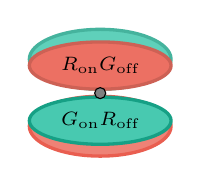
\begin{tikzpicture}
    \filldraw[color=greensea!80,    fill=turquoise!70, very thick]( 0.00, 1.43) ellipse   (0.90 and 0.38);
    \filldraw[color=alizarin!90,    fill=alizarin!70,  very thick]( 0.00, 0.58) ellipse   (0.90 and 0.38);
    \filldraw[color=pomegranate!80, fill=alizarin!80,  very thick]( 0.00, 1.35) ellipse   (0.90 and 0.30)
         node[color=black, anchor=center] {$\scriptstyle R_{\text{on}}G_{\text{off}}$};
    \filldraw[color=greensea,       fill=turquoise!80, very thick]( 0.00, 0.65) ellipse   (0.90 and 0.30)
         node[color=black, anchor=center] {$\scriptstyle G_{\text{on}}R_{\text{off}}$};
    \filldraw[color=black,          fill=gray]                    ( 0.00, 1.00) circle    (2pt);
\end{tikzpicture}



% FIGURE: horizontal red/green double-opponent cell on horizontal red/green border
\begin{figure}[h] \label{fig:do-orient-h}
    \begin{subfigure}{0.3\textwidth}
        \centering
        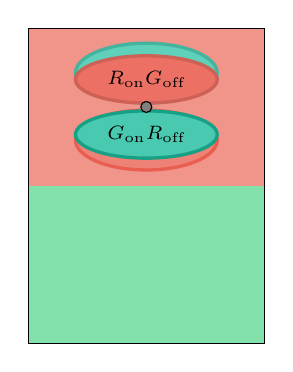
\begin{tikzpicture}
            \fill[alizarin!60]                                            (-1.50, 2.00) rectangle (1.50, 0.00);
            \fill[emerald!60]                                             (-1.50,-2.00) rectangle (1.50, 0.00);
            \filldraw[color=greensea!80,    fill=turquoise!70, very thick]( 0.00, 1.43) ellipse   (0.90 and 0.38);
            \filldraw[color=alizarin!90,    fill=alizarin!70,  very thick]( 0.00, 0.58) ellipse   (0.90 and 0.38);
            \filldraw[color=pomegranate!80, fill=alizarin!80,  very thick]( 0.00, 1.35) ellipse   (0.90 and 0.30)
                 node[color=black, anchor=center] {$\scriptstyle R_{\text{on}}G_{\text{off}}$};
            \filldraw[color=greensea,       fill=turquoise!80, very thick]( 0.00, 0.65) ellipse   (0.90 and 0.30)
                 node[color=black, anchor=center] {$\scriptstyle G_{\text{on}}R_{\text{off}}$};
            \filldraw[color=black,          fill=gray]                    ( 0.00, 1.00) circle    (2pt);
            \draw (current bounding box.north east) rectangle (current bounding box.south west);
        \end{tikzpicture}
        \caption{Minor Response}
    \end{subfigure}%
    \begin{subfigure}{0.3\textwidth}
        \centering
        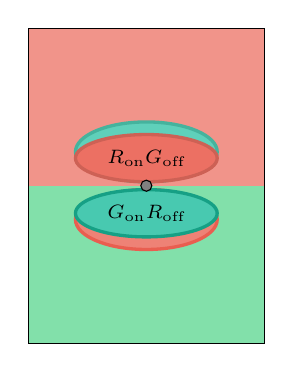
\begin{tikzpicture}
            \fill[alizarin!60]                                            (-1.50, 2.00) rectangle (1.50, 0.00);
            \fill[emerald!60]                                             (-1.50,-2.00) rectangle (1.50, 0.00);
            \filldraw[color=greensea!80,    fill=turquoise!70, very thick]( 0.00, 0.43) ellipse   (0.90 and 0.38);
            \filldraw[color=alizarin!90,    fill=alizarin!70,  very thick]( 0.00,-0.43) ellipse   (0.90 and 0.38);
            \filldraw[color=pomegranate!80, fill=alizarin!80,  very thick]( 0.00, 0.35) ellipse   (0.90 and 0.30)
                 node[color=black, anchor=center] {$\scriptstyle R_{\text{on}}G_{\text{off}}$};
            \filldraw[color=greensea,       fill=turquoise!80, very thick]( 0.00,-0.35) ellipse   (0.90 and 0.30)
                 node[color=black, anchor=center] {$\scriptstyle G_{\text{on}}R_{\text{off}}$};
            \filldraw[color=black,          fill=gray]                    ( 0.00, 0.00) circle    (2pt);
        \draw (current bounding box.north east) rectangle (current bounding box.south west);
        \end{tikzpicture}
        \caption{Maximum Response}
    \end{subfigure}%
    \begin{subfigure}{0.3\textwidth}
        \centering
        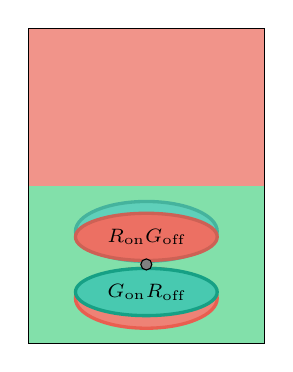
\begin{tikzpicture}
            \fill[alizarin!60]                                            (-1.50, 2.00) rectangle (1.50, 0.00);
            \fill[emerald!60]                                             (-1.50,-2.00) rectangle (1.50, 0.00);
            \filldraw[color=greensea!80,    fill=turquoise!70, very thick]( 0.00,-0.58) ellipse   (0.90 and 0.38);
            \filldraw[color=alizarin!90,    fill=alizarin!70,  very thick]( 0.00,-1.43) ellipse   (0.90 and 0.38);
            \filldraw[color=pomegranate!80, fill=alizarin!80,  very thick]( 0.00,-0.65) ellipse   (0.90 and 0.30)
                 node[color=black, anchor=center] {$\scriptstyle R_{\text{on}}G_{\text{off}}$};
            \filldraw[color=greensea,       fill=turquoise!80, very thick]( 0.00,-1.35) ellipse   (0.90 and 0.30)
                 node[color=black, anchor=center] {$\scriptstyle G_{\text{on}}R_{\text{off}}$};
            \filldraw[color=black,          fill=gray]                    ( 0.00,-1.00) circle    (2pt);
        \draw (current bounding box.north east) rectangle (current bounding box.south west);
        \end{tikzpicture}
        \caption{Minor Response}
    \end{subfigure}%
    \par \bigskip
    \begin{subfigure}{0.3\textwidth}
        \centering
        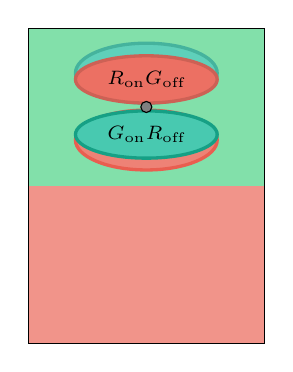
\begin{tikzpicture}
            \fill[emerald!60]                                             (-1.50, 2.00) rectangle (1.50, 0.00);
            \fill[alizarin!60]                                            (-1.50,-2.00) rectangle (1.50, 0.00);
            \filldraw[color=greensea!80,    fill=turquoise!70, very thick]( 0.00, 1.43) ellipse   (0.90 and 0.38);
            \filldraw[color=alizarin!90,    fill=alizarin!70,  very thick]( 0.00, 0.58) ellipse   (0.90 and 0.38);
            \filldraw[color=pomegranate!80, fill=alizarin!80,  very thick]( 0.00, 1.35) ellipse   (0.90 and 0.30)
                 node[color=black, anchor=center] {$\scriptstyle R_{\text{on}}G_{\text{off}}$};
            \filldraw[color=greensea,       fill=turquoise!80, very thick]( 0.00, 0.65) ellipse   (0.90 and 0.30)
                 node[color=black, anchor=center] {$\scriptstyle G_{\text{on}}R_{\text{off}}$};
            \filldraw[color=black,          fill=gray]                    ( 0.00, 1.00) circle    (2pt);
            \draw (current bounding box.north east) rectangle (current bounding box.south west);
        \end{tikzpicture}
        \caption{Minor Response}
    \end{subfigure}%
    \begin{subfigure}{0.3\textwidth}
        \centering
        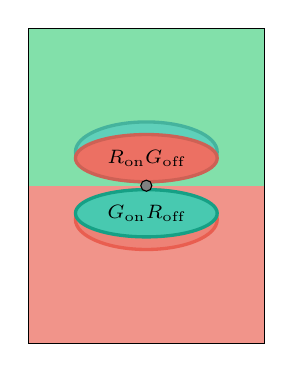
\begin{tikzpicture}
            \fill[emerald!60]                                             (-1.50, 2.00) rectangle (1.50, 0.00);
            \fill[alizarin!60]                                            (-1.50,-2.00) rectangle (1.50, 0.00);
            \filldraw[color=greensea!80,    fill=turquoise!70, very thick]( 0.00, 0.43) ellipse   (0.90 and 0.38);
            \filldraw[color=alizarin!90,    fill=alizarin!70,  very thick]( 0.00,-0.43) ellipse   (0.90 and 0.38);
            \filldraw[color=pomegranate!80, fill=alizarin!80,  very thick]( 0.00, 0.35) ellipse   (0.90 and 0.30)
                 node[color=black, anchor=center] {$\scriptstyle R_{\text{on}}G_{\text{off}}$};
            \filldraw[color=greensea,       fill=turquoise!80, very thick]( 0.00,-0.35) ellipse   (0.90 and 0.30)
                 node[color=black, anchor=center] {$\scriptstyle G_{\text{on}}R_{\text{off}}$};
            \filldraw[color=black,          fill=gray]                    ( 0.00, 0.00) circle    (2pt);
        \draw (current bounding box.north east) rectangle (current bounding box.south west);
        \end{tikzpicture}
        \caption{No Response}
    \end{subfigure}%
    \begin{subfigure}{0.3\textwidth}
        \centering
        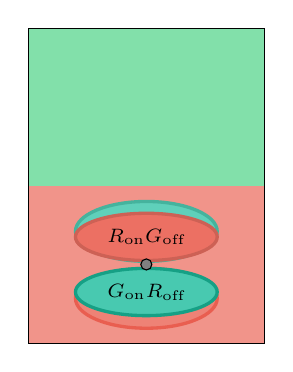
\begin{tikzpicture}
            \fill[emerald!60]                                             (-1.50, 2.00) rectangle (1.50, 0.00);
            \fill[alizarin!60]                                            (-1.50,-2.00) rectangle (1.50, 0.00);
            \filldraw[color=greensea!80,    fill=turquoise!70, very thick]( 0.00,-0.58) ellipse   (0.90 and 0.38);
            \filldraw[color=alizarin!90,    fill=alizarin!70,  very thick]( 0.00,-1.43) ellipse   (0.90 and 0.38);
            \filldraw[color=pomegranate!80, fill=alizarin!80,  very thick]( 0.00,-0.65) ellipse   (0.90 and 0.30)
                 node[color=black, anchor=center] {$\scriptstyle R_{\text{on}}G_{\text{off}}$};
            \filldraw[color=greensea,       fill=turquoise!80, very thick]( 0.00,-1.35) ellipse   (0.90 and 0.30)
                 node[color=black, anchor=center] {$\scriptstyle G_{\text{on}}R_{\text{off}}$};
            \filldraw[color=black,          fill=gray]                    ( 0.00,-1.00) circle    (2pt);
        \draw (current bounding box.north east) rectangle (current bounding box.south west);
        \end{tikzpicture}
        \caption{Minor Response}
    \end{subfigure}
    \caption{A double opponent cell selective to horizontally oriented borders with red above and green below; only responsive to that particular stimulus. In Figure (b), the neuron is presented with its ideal stimulus: its $R_{\text{on}}$ and $G_{\text{on}}$ receptive fields are fully activated while its $R_{\text{off}}$ and $G_{\text{off}}$ receptive fields are completely unactivated. Figure (e) presents the neuron with the exact opposite stimulus, neither its $R_{\text{on}}$ nor $G_{\text{on}}$ receptive fields are activate at all, and both its $R_{\text{off}}$ and $G_{\text{off}}$ receptive fields are fully activated, ensuring no response possible from the cell. While its $R_{\text{on}}$ receptive field might be strongly stimulated in (a) and (f), it's $R_{\text{off}}$ receptive field cancels it out. Similarly, in (c) and (d) its $G_{\text{on}}$ receptive field is stimulated but cancelled out by activity in its $G_{\text{off}}$ receptive field.}
\end{figure}

% FIGURE: vertical red/green double-opponent cell on horizontal red/green border
\begin{figure}[h] \label{fig:do-orient-v}
    \begin{subfigure}{0.3\textwidth}
        \centering
        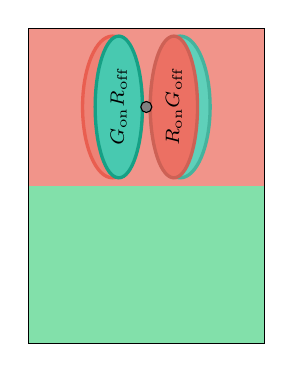
\begin{tikzpicture}
            \fill[alizarin!60]                                            (-1.50, 2.00) rectangle (1.50, 0.00);
            \fill[emerald!60]                                             (-1.50,-2.00) rectangle (1.50, 0.00);
            \filldraw[color=greensea!80,    fill=turquoise!70, very thick]( 0.43, 1.00) ellipse   (0.38 and 0.90);
            \filldraw[color=alizarin!90,    fill=alizarin!70,  very thick](-0.43, 1.00) ellipse   (0.38 and 0.90);
            \filldraw[color=pomegranate!80, fill=alizarin!80,  very thick]( 0.35, 1.00) ellipse   (0.30 and 0.90)
                 node[color=black, anchor=center, rotate=90] {$\scriptstyle R_{\text{on}}G_{\text{off}}$};
            \filldraw[color=greensea,       fill=turquoise!80, very thick](-0.35, 1.00) ellipse   (0.30 and 0.90)
                 node[color=black, anchor=center, rotate=90] {$\scriptstyle G_{\text{on}}R_{\text{off}}$};
            \filldraw[color=black,          fill=gray]                    ( 0.00, 1.00) circle    (2pt);
            \draw (current bounding box.north east) rectangle (current bounding box.south west);
        \end{tikzpicture}
        \caption{Minor Response}
    \end{subfigure}%
    \begin{subfigure}{0.3\textwidth}
        \centering
            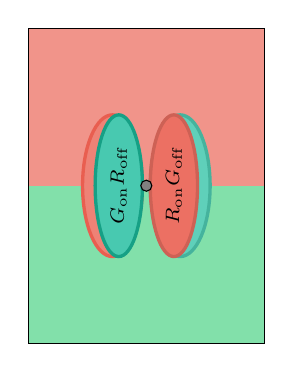
\begin{tikzpicture}
            \fill[alizarin!60]                                            (-1.50, 2.00) rectangle (1.50, 0.00);
            \fill[emerald!60]                                             (-1.50,-2.00) rectangle (1.50, 0.00);
            \filldraw[color=greensea!80,    fill=turquoise!70, very thick]( 0.43, 0.00) ellipse   (0.38 and 0.90);
            \filldraw[color=alizarin!90,    fill=alizarin!70,  very thick](-0.43, 0.00) ellipse   (0.38 and 0.90);
            \filldraw[color=pomegranate!80, fill=alizarin!80,  very thick]( 0.35, 0.00) ellipse   (0.30 and 0.90)
                 node[color=black, anchor=center, rotate=90] {$\scriptstyle R_{\text{on}}G_{\text{off}}$};
            \filldraw[color=greensea,       fill=turquoise!80, very thick](-0.35, 0.00) ellipse   (0.30 and 0.90)
                 node[color=black, anchor=center, rotate=90] {$\scriptstyle G_{\text{on}}R_{\text{off}}$};
            \filldraw[color=black,          fill=gray]                    ( 0.00, 0.00) circle    (2pt);
            \draw (current bounding box.north east) rectangle (current bounding box.south west);
            \end{tikzpicture}
        \caption{Minimal Response}
    \end{subfigure}%
    \begin{subfigure}{0.3\textwidth}
        \centering
            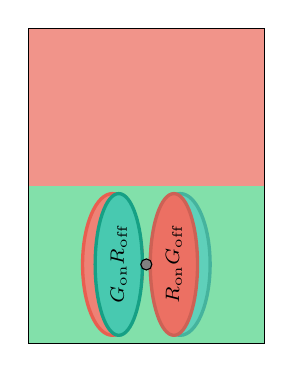
\begin{tikzpicture}
            \fill[alizarin!60]                                            (-1.50, 2.00) rectangle (1.50, 0.00);
            \fill[emerald!60]                                             (-1.50,-2.00) rectangle (1.50, 0.00);
            \filldraw[color=greensea!80,    fill=turquoise!70, very thick]( 0.43,-1.00) ellipse   (0.38 and 0.90);
            \filldraw[color=alizarin!90,    fill=alizarin!70,  very thick](-0.43,-1.00) ellipse   (0.38 and 0.90);
            \filldraw[color=pomegranate!80, fill=alizarin!80,  very thick]( 0.35,-1.00) ellipse   (0.30 and 0.90)
                 node[color=black, anchor=center, rotate=90] {$\scriptstyle R_{\text{on}}G_{\text{off}}$};
            \filldraw[color=greensea,       fill=turquoise!80, very thick](-0.35,-1.00) ellipse   (0.30 and 0.90)
                 node[color=black, anchor=center, rotate=90] {$\scriptstyle G_{\text{on}}R_{\text{off}}$};
            \filldraw[color=black,          fill=gray]                    ( 0.00,-1.00) circle    (2pt);
            \draw (current bounding box.north east) rectangle (current bounding box.south west);
            \end{tikzpicture}
        \caption{Minor Response}
    \end{subfigure}%
    \par \bigskip
    \begin{subfigure}{0.3\textwidth}
        \centering
        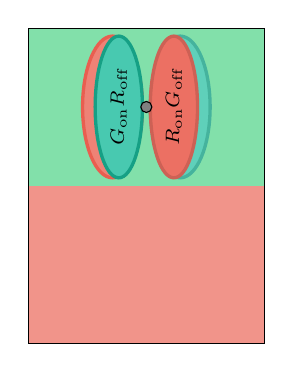
\begin{tikzpicture}
            \fill[emerald!60]                                             (-1.50, 2.00) rectangle (1.50, 0.00);
            \fill[alizarin!60]                                            (-1.50,-2.00) rectangle (1.50, 0.00);
            \filldraw[color=greensea!80,    fill=turquoise!70, very thick]( 0.43, 1.00) ellipse   (0.38 and 0.90);
            \filldraw[color=alizarin!90,    fill=alizarin!70,  very thick](-0.43, 1.00) ellipse   (0.38 and 0.90);
            \filldraw[color=pomegranate!80, fill=alizarin!80,  very thick]( 0.35, 1.00) ellipse   (0.30 and 0.90)
                 node[color=black, anchor=center, rotate=90] {$\scriptstyle R_{\text{on}}G_{\text{off}}$};
            \filldraw[color=greensea,       fill=turquoise!80, very thick](-0.35, 1.00) ellipse   (0.30 and 0.90)
                 node[color=black, anchor=center, rotate=90] {$\scriptstyle G_{\text{on}}R_{\text{off}}$};
            \filldraw[color=black,          fill=gray]                    ( 0.00, 1.00) circle    (2pt);
            \draw (current bounding box.north east) rectangle (current bounding box.south west);
        \end{tikzpicture}
        \caption{Minor Response}
    \end{subfigure}%
    \begin{subfigure}{0.3\textwidth}
        \centering
            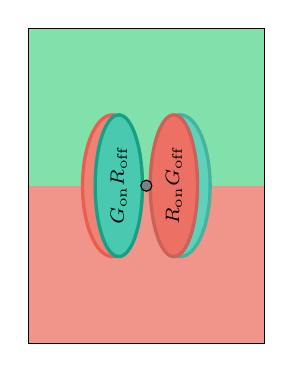
\begin{tikzpicture}
            \fill[emerald!60]                                             (-1.50, 2.00) rectangle (1.50, 0.00);
            \fill[alizarin!60]                                            (-1.50,-2.00) rectangle (1.50, 0.00);
            \filldraw[color=greensea!80,    fill=turquoise!70, very thick]( 0.43, 0.00) ellipse   (0.38 and 0.90);
            \filldraw[color=alizarin!90,    fill=alizarin!70,  very thick](-0.43, 0.00) ellipse   (0.38 and 0.90);
            \filldraw[color=pomegranate!80, fill=alizarin!80,  very thick]( 0.35, 0.00) ellipse   (0.30 and 0.90)
                 node[color=black, anchor=center, rotate=90] {$\scriptstyle R_{\text{on}}G_{\text{off}}$};
            \filldraw[color=greensea,       fill=turquoise!80, very thick](-0.35, 0.00) ellipse   (0.30 and 0.90)
                 node[color=black, anchor=center, rotate=90] {$\scriptstyle G_{\text{on}}R_{\text{off}}$};
            \filldraw[color=black,          fill=gray]                    ( 0.00, 0.00) circle    (2pt);
            \draw (current bounding box.north east) rectangle (current bounding box.south west);
            \end{tikzpicture}
        \caption{Minimal Response}
    \end{subfigure}%
    \begin{subfigure}{0.3\textwidth}
        \centering
            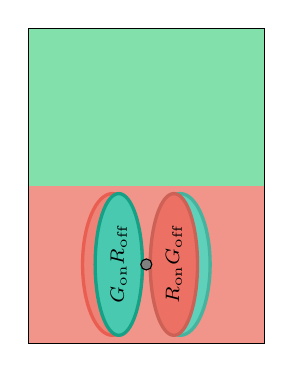
\begin{tikzpicture}
            \fill[emerald!60]                                             (-1.50, 2.00) rectangle (1.50, 0.00);
            \fill[alizarin!60]                                            (-1.50,-2.00) rectangle (1.50, 0.00);
            \filldraw[color=greensea!80,    fill=turquoise!70, very thick]( 0.43,-1.00) ellipse   (0.38 and 0.90);
            \filldraw[color=alizarin!90,    fill=alizarin!70,  very thick](-0.43,-1.00) ellipse   (0.38 and 0.90);
            \filldraw[color=pomegranate!80, fill=alizarin!80,  very thick]( 0.35,-1.00) ellipse   (0.30 and 0.90)
                 node[color=black, anchor=center, rotate=90] {$\scriptstyle R_{\text{on}}G_{\text{off}}$};
            \filldraw[color=greensea,       fill=turquoise!80, very thick](-0.35,-1.00) ellipse   (0.30 and 0.90)
                 node[color=black, anchor=center, rotate=90] {$\scriptstyle G_{\text{on}}R_{\text{off}}$};
            \filldraw[color=black,          fill=gray]                    ( 0.00,-1.00) circle    (2pt);
            \draw (current bounding box.north east) rectangle (current bounding box.south west);
            \end{tikzpicture}
        \caption{Minor Response}
    \end{subfigure}
    \caption{A double opponent cell selective to vertically oriented borders with red to the right and green on the left; completely unresponsive to a horizontal border. While its $R_{\text{on}}$ receptive field might be strongly stimulated in (a) and (f), it's $R_{\text{off}}$ receptive field cancels it out. Similarly, in (c) and (d) its $G_{\text{on}}$ receptive field is stimulated but cancelled out by activity in its $G_{\text{off}}$ receptive field. In (b) and (e) both of its $R_{\text{on}}$ and $G_{\text{on}}$ receptive fields are moderately activated, but again, cancelled out by activation in its $R_{\text{off}}$ and $G_{\text{off}}$ receptive fields, respectively.}
\end{figure}

\end{document}